\documentclass[10pt]{beamer}
% \documentclass[handout,10pt]{beamer}
\usepackage{my_style}

\title[Math/CS 375]{Lecture 09 - C}
\subtitle{\S 4.2,6.1 Interpolation Error}


\begin{document}
% -------------------------------------------------
\begin{frame}
  \titlepage
\end{frame}
% -------------------------------------------------
\begin{frame}{Goals}
We will answer these questions:\\[3mm]
\begin{itemize}
    \item How well does interpolation approximate a function?
    \item When does polynomial interpolation lead to disaster? 
    \item What are Chebyshev nodes and how are they related to interpolation?
    \item What are splines? In what way are they advantageous over standard polynomial interpolation?
\end{itemize}
\end{frame}


%%%%%%%%%%%%%%%%%%%%%%%%%%%%%%%%%%%%%%%%%%%%%%%%%%%%%%%%%%%%%%%%%%%%%%%%
\begin{frame}{Quantifying Error for Interpolation}

{\question{
    How can we quantify how well of an interpolation $p(x)$ approximates the unknown function $f(x)$?
}}

\begin{block}{}
    In polynomial interpolation, we assume that the data points $(x_i,y_i)$ come from some unknown continuous function $f(x)$
\end{block}

\begin{block}{}
    \textbf{Simple answer:} We can choose our own function $f(x)$ and create our data points  $e(x)=f(x)-p_n(x)$. 
\end{block}
\end{frame}

%%%%%%%%%%%%%%%%%%%%%%%%%%%%%%%%%%%%%%%%%%%%%%%%%%%%%%%%%%%%%%%%%%%%%%%%

\begin{frame}{Quantifying Error for Interpolation}{Strategy}
Strategy for quantifying error : 
\begin{enumerate}
    \item Choose a function $f(x)$

    \item Choose $n+1$ values of $x$ to get the $x_i$

    \item Generate data points $(x_i,y_i)$ where $y_i =f(x_i)$

    \item Interpolate $(x_i,y_i)$ to get our polynomial $p(x)$

    \item Calculate the error $e(x) = f(x) - p(x)$
\end{enumerate}

\vspace{5mm}
{
\define{Sampling}{
Extracting the value of $y=f(x)$ at finite discrete points is called \textbf{sampling}.
}
}

\question{How do choose the sample points?}

\end{frame}


\begin{frame}[fragile]{Evenly Distributed Sample Points}
\begin{itemize}
\item To get $n+1$ equally spread out over $[a,b]$, we first break up $[a,b]$ into $n$ subintervals $$h = \frac{b-a}{n}$$
\item The first point is always $x_0=a$ and the last is always $x_{n+1}=b$
\item The points in between are given by $x_i = x_0 + ih$
\method{Equispaced Discretization}{Interval $[a,b]$, Number of points $n+1$}{Set of equally spaced out points $\{x_i\}$}{Use the constant space $h=(b-a)/n$ to determine the points.}
\item In Matlab, this is simply 
\end{itemize}
\begin{lstlisting} 
>> xx = linspace(a,b,n+1);
\end{lstlisting} 
\end{frame}

%-------------------------------------

\begin{frame}{Discretization Example}

\begin{example}
    Discretize the interval $[0,1]$ into equispaced 5 points. 
\end{example}

\begin{itemize}
    \item Left-end $a=0$ and right-end $b=1$ are included as part of the 5 points.
    \item Number of subintervals is  $n=5-1=4$.
    \item Can be helpful to draw the line interval \\[7mm] 
\begin{center}    
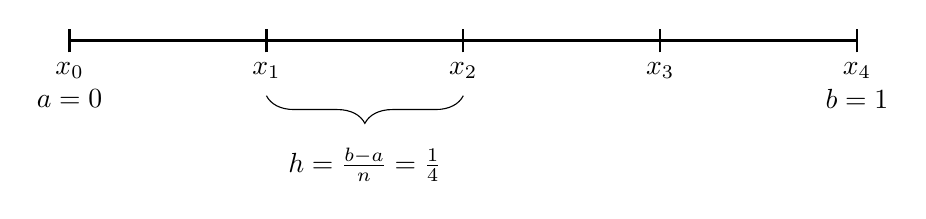
\begin{tikzpicture}
    % Define interval length
    \def\IntervalLength{10}
    \def\n{4}  % Number of subintervals
    \def\dx{\IntervalLength/\n}  % Length of each subinterval

    % Draw the interval
    \draw[thick] (0,0) -- (\IntervalLength,0);

    % Draw nodes and labels
    \foreach \i in {0,...,\n} {
        \draw[thick] ({\i*\dx},-0.15) -- ({\i*\dx},0.15);  % Vertical tick marks
        \node[below] at ({\i*\dx},-0.15) {$x_\i$};  % Node labels
    }
    % Optional: Label the interval's ends
    \node[below] at (0,-0.5) {$a=0$};
    \node[below] at (\IntervalLength,-0.5) {$b=1$};

    \draw [decorate,decoration={brace,amplitude=10pt}] ({2*\dx},-0.7) -- ({1*\dx},-0.7) 
        node [midway,yshift=-25pt] {$h = \frac{b-a}{n} = \frac{1}{4}$};

\end{tikzpicture}
\end{center}
    \item Based on the drawing, our discretization is $\{0, 0.25, 0.5, 0.75, 1.0\}$
    \item We can also use the formula $x_k= x_0 + h\,k=0 + 0.25\,k$

\end{itemize}
\end{frame}

%-----------------------------------
\subsection{Visual Error}
%-----------------------------------

\begin{frame}{Original vs. Interpolation}

    \begin{itemize}
        \item Let $f(x)$ be our test function sampled on $[a,b]$ 

        \item Leg $g(x)$ be our interpolation using data from $(a,(f(a)),\dots,(b,f(b))$

        \begin{block}{Visual Error}
            Plot $f(x)$ and $g(x)$ together and see the difference.
        \end{block}

        \begin{block}{Max Discrepancy}
            We may define 
            $$
                E = \max_{x\in(a,b)} |f(x)-p(x)|
            $$
        \end{block}
    \end{itemize}

\end{frame}


\begin{frame}[fragile]{Interpolate $y=\sin(x)$ with $n=4$}
\cols{
\begin{itemize}
    \item Consider sampling $f(x)=\sin(x)$ over $[0,2\pi]$ with
        $n = 4$
    \item Interpolation is roughly
    $$p(x) \approx 1.697 x - 0.8106x^2 + 0.086 x^3 $$
    \item There is visual difference between the true function (blue curve) and the interpolation (dashed curve) 
\end{itemize}
}
{
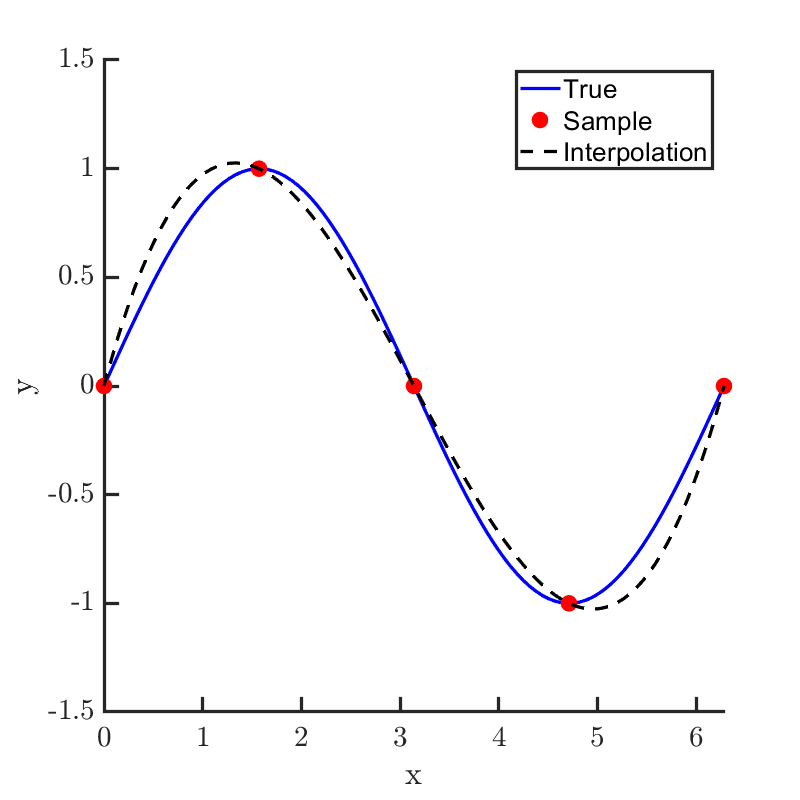
\includegraphics[width=\textwidth]{figs/interp_n4.png}
}    
\end{frame}
%-------------------------------------
\begin{frame}[fragile]{Interpolate $y=\sin(x)$ with $n=8$}
\cols{
\begin{itemize}
    \item Same interpolation with 
        $$n = 8$$
    \item No visual error on $[0,\pi]$! 

    \item $n=8$ looks better than $n=4$
\end{itemize}
}
{
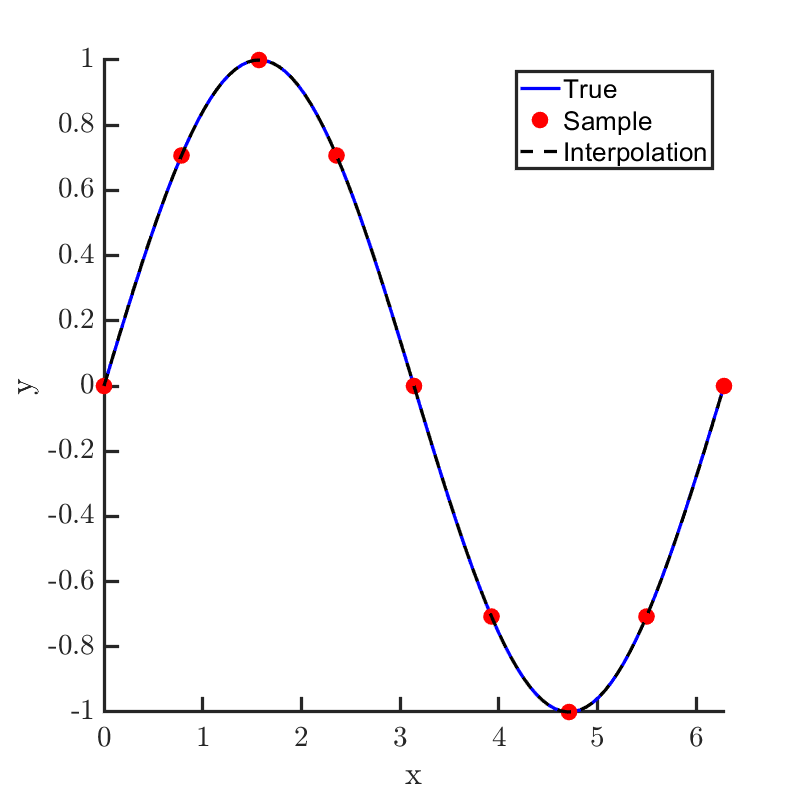
\includegraphics[width=\textwidth]{figs/interp_n8.png}
}    

\begin{itemize}
    \item Logic says

$$ \text{increase } n \Rightarrow \text{use more information} \Rightarrow \text{decrease error}$$
\end{itemize}

\end{frame}
%-------------------------------------
\begin{frame}{Beyond the Sample Points}

\begin{itemize}
    \item We sampled $\sin(x)$ only on $[0,\pi]$.
    \item What happens if we evaluate the polynomial beyond $\pi$?
\end{itemize}

\begin{center}
    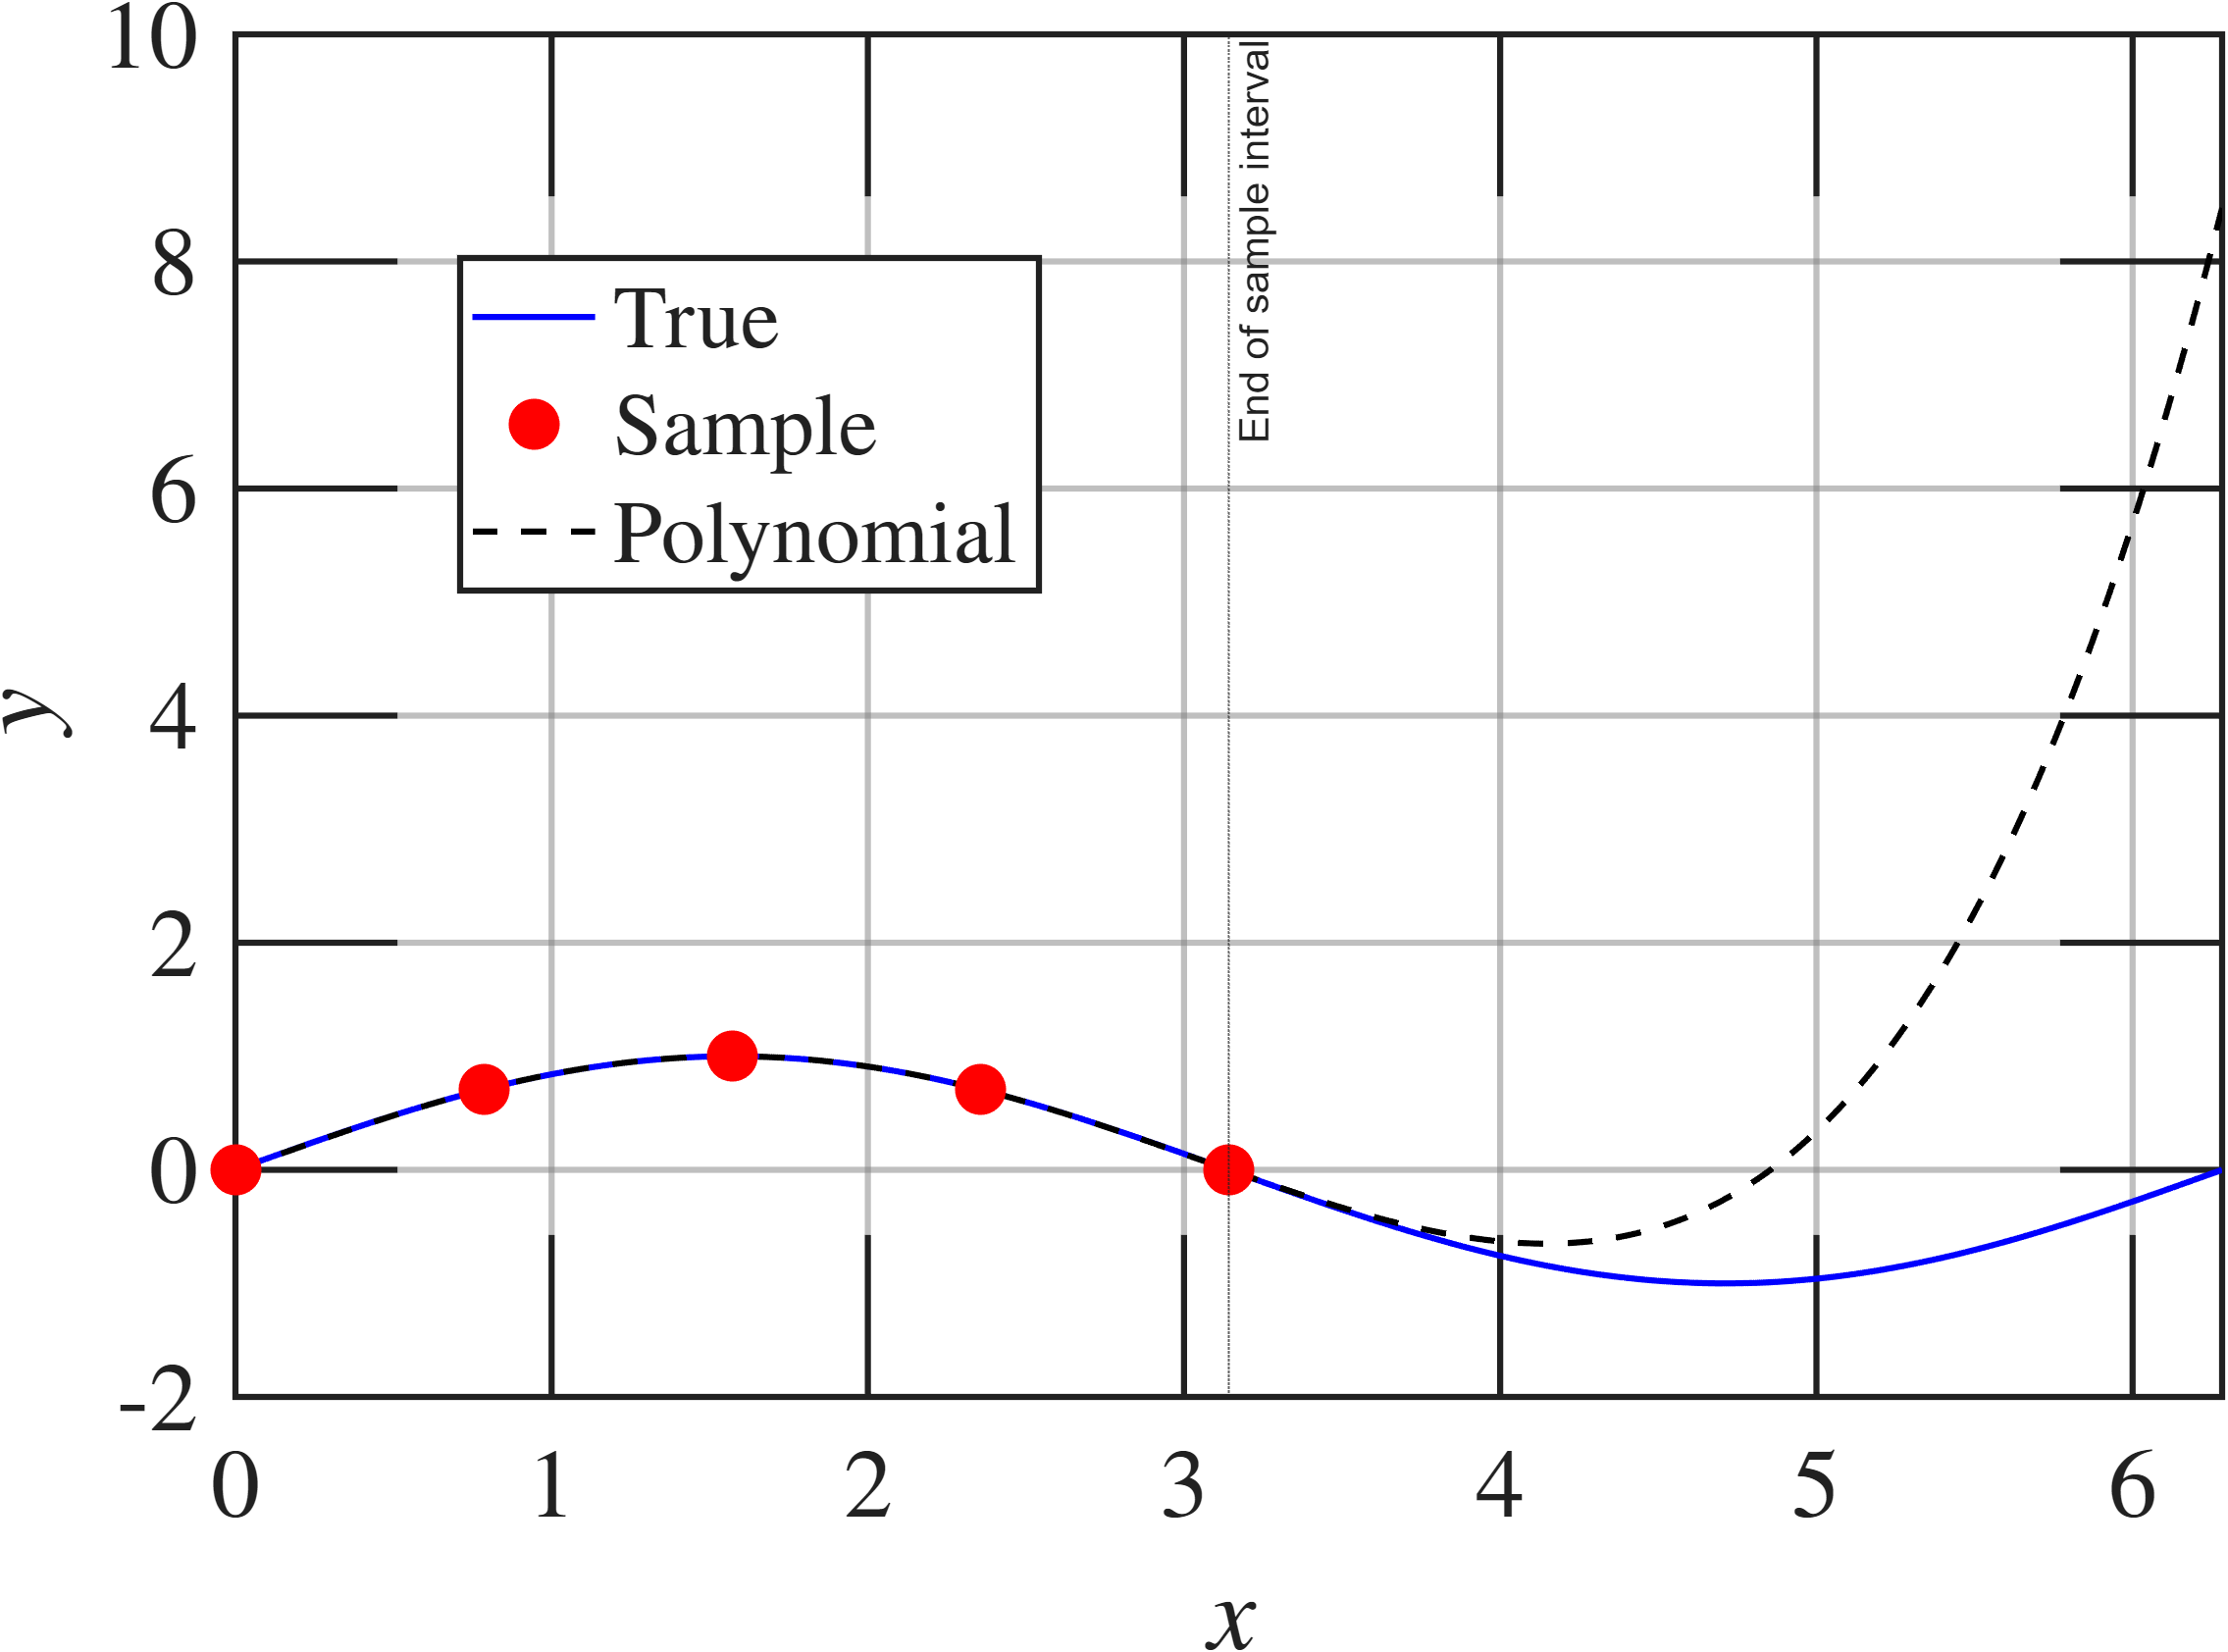
\includegraphics[width=0.7\linewidth]{figs/sine_extrapolation.png}
\end{center}



\end{frame}

%-------------------------------------
%%%%%%%%%%%%%%%%%%%%%%%%%%%%%%%%%%%%%%%%%%%
\begin{frame}{Interpolation vs. Extrapolation}

\begin{block}{Interpolation}
Estimate values \textbf{inside} the sampled interval:
\[
    x\in[x_0,x_n].
\]
\end{block}

\begin{block}{Extrapolation}
Estimate values \textbf{outside} the sampled interval:
\[
    x<x_0 \qquad \text{or} \qquad x>x_n.
\]
\end{block}

\begin{itemize}
    \item The same polynomial can be evaluated in either region.
    \item A good fit inside the interval does not guarantee
    accuracy outside it.
\end{itemize}

\onslide<2->{
\keyidea{
The polynomial approximation $p(x)\approx f(x)$ is only valid in the data range
}
}

\end{frame}

%-------------------------------------



\begin{frame}{Case Study: Runge Function}
Consider \textbf{Runge function}
  \[
  f(x) = \frac{1}{1 + 25x^2}
  \]
\cols{
Properties:
\begin{itemize}
\item no singularities - \textit{good}
\item bounded - \textit{good}
\item smooth - \textit{good}
\item We write this as $f\in C^{\infty}_b(\mathbb{R})$
\end{itemize}
}{
\begin{center}    
  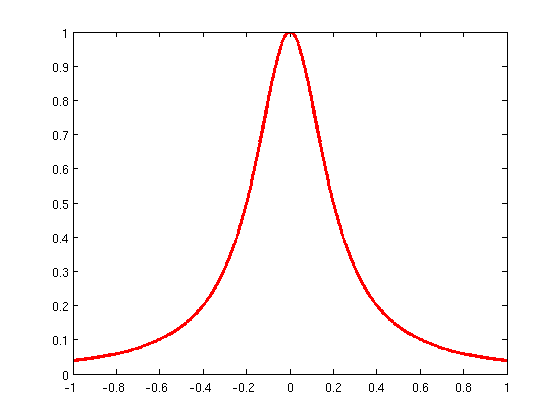
\includegraphics[width=\textwidth]{./figs/runge}\\
\end{center}
}
\question{  
Runge's function is very nice on paper. How well does equispaced interpolation capture the function?
}

\end{frame}

%%%%%%%%%%%%%%%%%%%%%%%%%%%%%%%%%%%%%%%%%%%%%%%%%%%%%%%%%%%
\begin{frame}{Case Study: Runge Function}{Interpolation results}
\begin{equation*}
  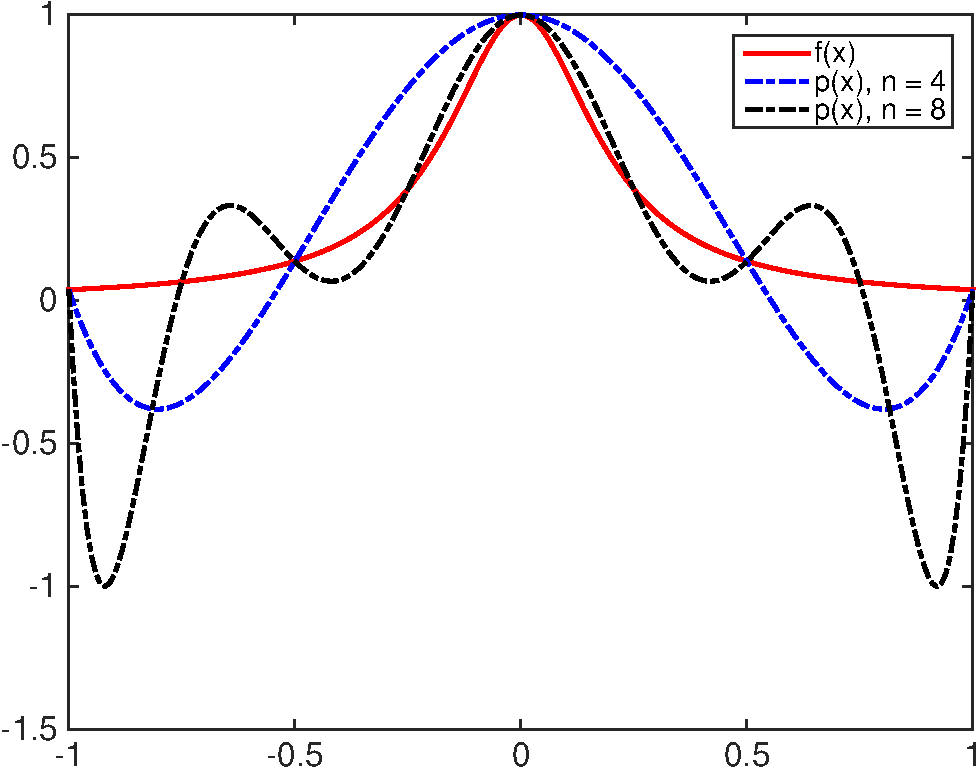
\includegraphics[height=4.5cm]{./figs/runge_interp}
\end{equation*}

\medskip

\textbf{Answer:} Not very well\smallskip
\begin{itemize}
% \item We were expecting to see $p_4(x) \approx f(x)$ and $p_8(x)\approx f(x)$
\item $p_4(x)$ using 5 nodes looks bad 
\item $p_8(x)$ using 9 nodes \textit{looks even worse} 
\item $p_n(x)$ will continue to worsen as $n$ is increased

% \item Can show that, when using equispaced interpolatory points, 
% \[
% \lim_{n \rightarrow \infty} \left (  \max_{-1 \leq x \leq 1} |f(x) - p_n(x)| = \infty \right)
% \]
\end{itemize}
\end{frame}
%%%%%%%%%%%%%%%%%%%%%%%%%%%%%%%%%%%%%%%%%%%%%%%%%%%%%%%%%%%
\begin{frame}{Case Study: Runge Function}{What went wrong?}
\vspace{-10mm}
\cols{
\begin{center}
$$f(x) = \sin(x)$$
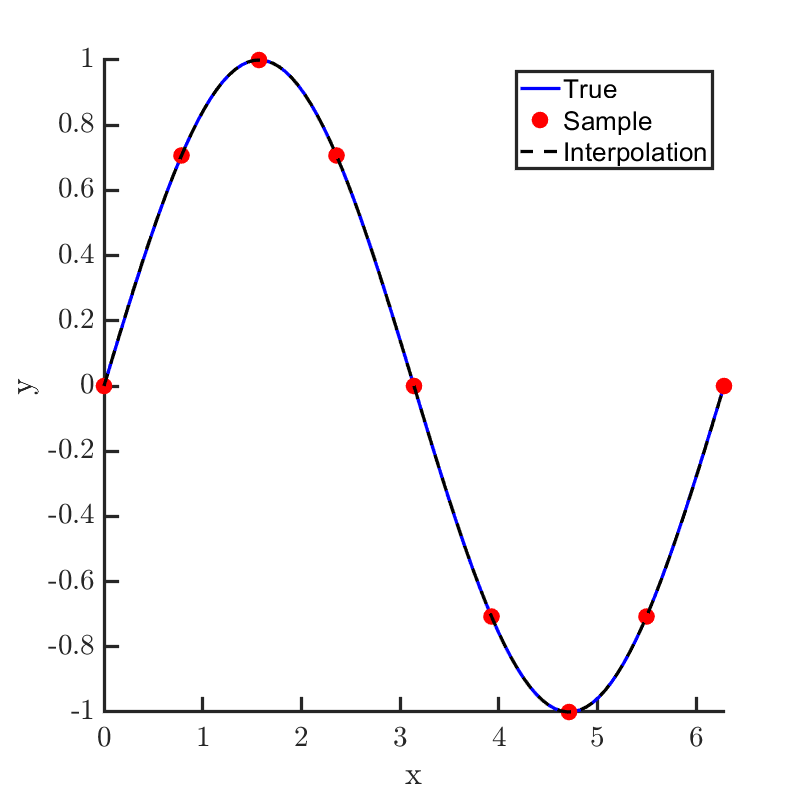
\includegraphics[width=\textwidth]{figs/interp_n8.png}\\
No visible error
\end{center}

}{
\begin{center}
$$f(x) = \frac{1}{1+25x^2}$$
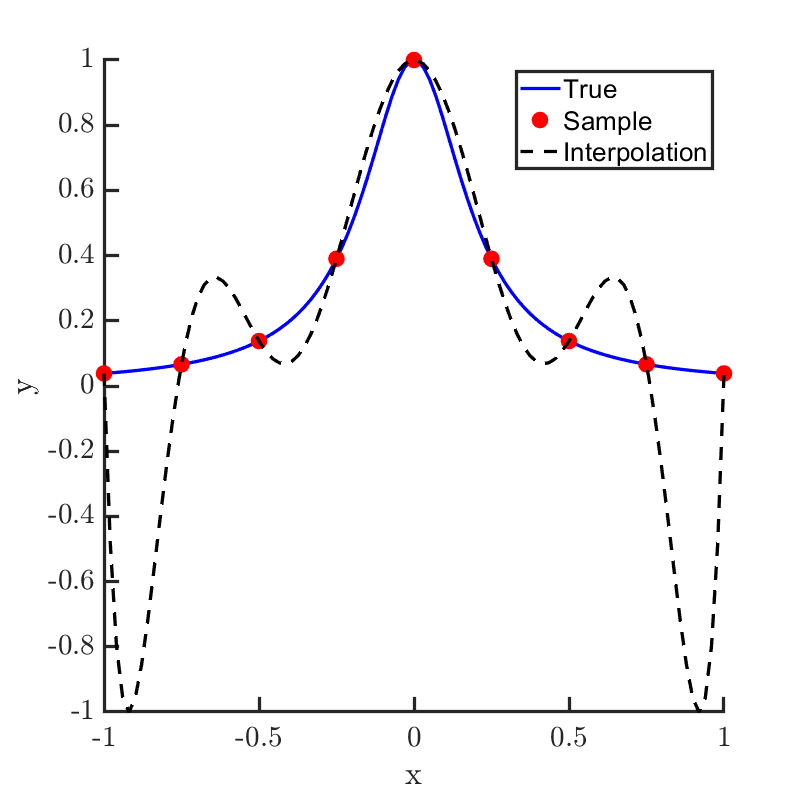
\includegraphics[width=\textwidth]{figs/interp_n8_runge.png}
Very inaccurate
\end{center}
}
    
\end{frame}
%%%%%%%%%%%%%%%%%%%%%%%%%%%%%%%%%%%%%%%%%%%%%%%%%%%%%%%%%%
\sectionframe{Interpolation Error}
%%%%%%%%%%%%%%%%%%%%%%%%%%%%%%%%%%%%%%%%%%%%%%%%%%%%%%%%%%
\begin{frame}{Rolle's Theorem}
\begin{block}{Theorem}
    If $f(a)=f(b)$ then $\exists c\in(a,b)$ such that $f'(c)=0$.
\end{block}

\begin{figure}[h]
\centering
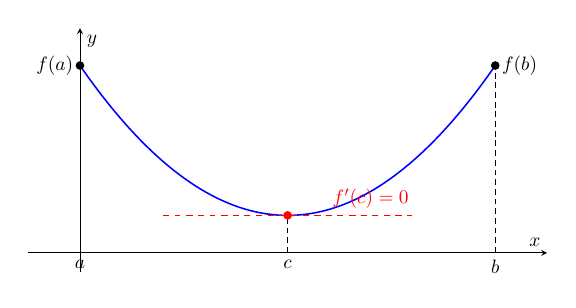
\begin{tikzpicture}[scale=0.7]
\begin{axis}[
    width=11cm,
    height=6cm,
    axis lines=middle,
    xmin=-0.5, xmax=4.5,
    ymin=-0.5, ymax=6,
    xtick=\empty,
    ytick=\empty,
    xlabel={$x$},
    ylabel={$y$},
    domain=0:4,
    samples=200,
    clip=false
]

% quadratic curve
\addplot[thick, blue] {(x-2)^2 + 1};

% endpoints a and b
\addplot[only marks, mark=*, mark size=2pt] coordinates {(0,5) (4,5)};
\node[below] at (axis cs:0,0) {$a$};
\node[below] at (axis cs:4,0) {$b$};

% labels for endpoint values
\node[left] at (axis cs:0,5) {$f(a)$};
\node[right] at (axis cs:4,5) {$f(b)$};

% point c
\addplot[only marks, mark=*, mark size=2pt, red] coordinates {(2,1)};
\node[below] at (axis cs:2,0) {$c$};

% flat tangent line at c
\addplot[dashed, red, domain=0.8:3.2] {1};
\node[above, red] at (axis cs:2.8,1) {$f'(c)=0$};

% dashed vertical guides
\addplot[densely dashed] coordinates {(0,0) (0,5)};
\addplot[densely dashed] coordinates {(4,0) (4,5)};
\addplot[densely dashed] coordinates {(2,0) (2,1)};
\end{axis}
\end{tikzpicture}
\end{figure}

\keyidea{If $f(x)$ returns to the same value, then at some point, it must have turned around.}

\end{frame}
\begin{frame}{Two-Point Interpolation}
    \begin{figure}[h]
\centering
\begin{tikzpicture}
\begin{axis}[
    width=11cm,
    height=6cm,
    axis lines=middle,
    xmin=-0.5, xmax=5.5,
    ymin=0, ymax=6,
    xlabel={$x$},
    ylabel={$y$},
    xtick=\empty,
    ytick=\empty,
    samples=200,
    domain=0:5,
    clip=false
]

% function
\addplot[thick, blue] {x + cos(deg(x))};


% chosen interpolation points
\addplot[only marks, mark=*, mark size=2pt] 
coordinates {
    (1,{1 + cos(deg(1))})
    (4,{4 + cos(deg(4))})
};

\node[above left] at (axis cs:1,{1 + cos(deg(1))}) {$\bigl(x_0,f(x_0)\bigr)$};
\node[above right] at (axis cs:4,{4 + cos(deg(4))}) {$\bigl(x_1,f(x_1)\bigr)$};

% secant line through the two points
\addplot[dashed, red, domain=0.4:4.6]
{(1 + cos(deg(1))) 
+ ((4 + cos(deg(4))) - (1 + cos(deg(1))))/(4-1) * (x-1)};



% vertical guides
\addplot[densely dashed, gray] coordinates {(1,0) (1,{1 + cos(deg(1))})};
\addplot[densely dashed, gray] coordinates {(4,0) (4,{4 + cos(deg(4))})};

\node[below] at (axis cs:1,0) {$x_0$};
\node[below] at (axis cs:4,0) {$x_1$};

\end{axis}
\end{tikzpicture}
\end{figure}

\begin{block}{Interpolation}
    Let $f(x)$ be the actual function. Let $p_1(x)$ be the two-point interpolation of $f(x)$.
\end{block}
\end{frame}
%%%%%%%%%%%%%%%%%%%%%%%%%%%%%%%%%%%%%%%%%%%%%%%%%%%%%%%%%%

\begin{frame}{Some analysis...}
\begin{block}{Interpolation Error}
    $$
    e(x) = f(x) - p_1(x)
    $$
\end{block}

\begin{block}{Consider this function}
    \begin{equation*}
  g(t) := e(t) - \frac{(t-x_0)(t-x_1)}{(x-x_0)(x-x_1)}e(x)
\end{equation*}
Notice that
\begin{itemize}
    \item $g(x_0)=0$
    \item $g(x_1)=0$
    \item $g(x)=0$
\end{itemize}
\end{block}

\end{frame}
%%%%%%%%%%%%%%%%%%%%%%%%%%%%%%%%%%%%%%%%
\begin{frame}{Using Rolle's Theorem}

\begin{block}{Consider this function}
    \begin{equation*}
  g(t) := e(t) - \frac{(t-x_0)(t-x_1)}{(x-x_0)(x-x_1)}e(x)
\end{equation*}
\end{block}


Since $g(t)=0$ at $t=x_0, x_1, x$
\begin{itemize}
  \item That implies $g'(t)$ is zero at \textbf{two} points 
  \item That implies $g''(t)$ is zero at \textbf{one} point; call it $c$
  \item Then
\begin{align*}
  0 & = g''(c) = e''(c) - 2 \frac{e(x)}{(x-x_0)(x-x_1)}\\
    & = f''(c) - 2 \frac{e(x)}{(x-x_0)(x-x_1)}\\
  e(x) &= \frac{(x-x_0)(x-x_1)}{2} f''(c)
\end{align*}
\end{itemize}
\end{frame}

%%%%%%%%%%%%%%%%%%%%%%%%%%%%%%%%%%%%%%%%
\begin{frame}{Error Formula for Two Points}

\begin{block}{Result}
    Suppose $f(x)$ is approximated by an interpolation $p_1(x)$ at two points $x_0$ and $x_1$. The error is given by 
    $$
    e(x) = f(x)-p_1(x) = \frac{(x-x_0)(x-x_1)}{2} f''(c)
    $$
\end{block}
\begin{figure}[h]
\centering
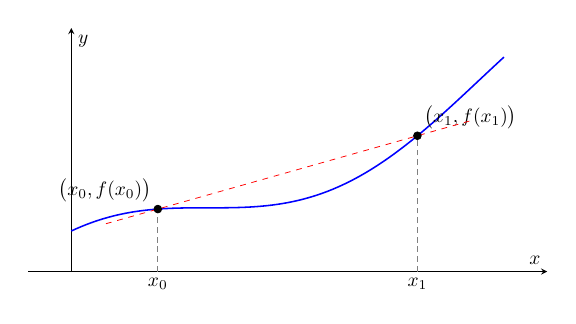
\begin{tikzpicture}[scale=0.7]
\begin{axis}[
    width=11cm,
    height=6cm,
    axis lines=middle,
    xmin=-0.5, xmax=5.5,
    ymin=0, ymax=6,
    xlabel={$x$},
    ylabel={$y$},
    xtick=\empty,
    ytick=\empty,
    samples=200,
    domain=0:5,
    clip=false
]

% function
\addplot[thick, blue] {x + cos(deg(x))};


% chosen interpolation points
\addplot[only marks, mark=*, mark size=2pt] 
coordinates {
    (1,{1 + cos(deg(1))})
    (4,{4 + cos(deg(4))})
};

\node[above left] at (axis cs:1,{1 + cos(deg(1))}) {$\bigl(x_0,f(x_0)\bigr)$};
\node[above right] at (axis cs:4,{4 + cos(deg(4))}) {$\bigl(x_1,f(x_1)\bigr)$};

% secant line through the two points
\addplot[dashed, red, domain=0.4:4.6]
{(1 + cos(deg(1))) 
+ ((4 + cos(deg(4))) - (1 + cos(deg(1))))/(4-1) * (x-1)};

% vertical guides
\addplot[densely dashed, gray] coordinates {(1,0) (1,{1 + cos(deg(1))})};
\addplot[densely dashed, gray] coordinates {(4,0) (4,{4 + cos(deg(4))})};

\node[below] at (axis cs:1,0) {$x_0$};
\node[below] at (axis cs:4,0) {$x_1$};

\end{axis}
\end{tikzpicture}
\end{figure}

\end{frame}
%%%%%%%%%%%%%%%%%%%%%%%%%%%%%%%%%%%%%%%%
\begin{frame}{And if there were 3 points...}

\question{What's the error for a three-point interpolation?}
\begin{itemize}
\item For 3 points, the error is still
\begin{equation*}
  e(x) = f(x) - p_2(x)
\end{equation*}

  \item For this case, we let 
\begin{equation*}
  g(t) := e(t) - \frac{(t-x_0)(t-x_1)(t-x_2)}{(x-x_0)(x-x_1)(x-x_2)}e(x)
\end{equation*}
  \item Then we take 3 derivatives and find that
\begin{align*}
  e(x) &= \frac{(x-x_0)(x-x_1)(x-x_2)}{6} f'''(c)
\end{align*}
\item<2> This is generalizable to any number of points!
\end{itemize}
\end{frame}

%%%%%%%%%%%%%%%%%%%%%%%%%%%%%%%%%%%%%%%%
\begin{frame}{Analysis of Interpolation Error: General Result}
\vspace{-0.5cm}
\begin{block}{Theorem: Interpolation Error I}
  If $p_n(x)$ is the (at most) $n$ degree polynomial interpolating $f(x)$ at
$n+1$ distinct points and if $f^{(n+1)}$ is continuous, then 
\begin{equation*}
  e(x) = f(x) - p_n(x) = \frac{f^{(n+1)}(c)}{(n+1)!}  \prod_{i=0}^{n}(x-x_i)
\end{equation*}
\end{block}
Proof in the book NMC 7th page 181.

\vspace{4ex}
\begin{itemize}
    \item At a glance, it looks like the error decreases like $O(\frac{1}{n!})$ (that's extremely fast!)
    \item So why did the error Runge's function grow? 
    \item That last term $\prod_{i=0}^{n}(x-x_i)$ doesn't depend on $f$. Just how large is it?
\end{itemize}
\end{frame}

%%%%%%%%%%%%%%%%%%%%%%%

\begin{frame}{Product Term}

\begin{block}{Interpolation error formula}
\[
f(x)-p_n(x)=\frac{f^{(n+1)}(\xi_x)}{(n+1)!}\prod_{i=0}^n (x-x_i)
\]
\end{block}

\pause

\keyidea{
The product term
\[
\prod_{i=0}^n (x-x_i)
\]
depends only on the location of the interpolation points.
}

\pause

\begin{itemize}
    \item Each factor $(x-x_i)$ is the distance from $x$ to the node $x_i$
    \item So the error is small when these distances are small
\end{itemize}
\end{frame}

\begin{frame}{Equally spaced nodes on a fixed interval}

{
\question{What if assume the points $x_i$ are equispaced:
\[
x_i=a+ih, \qquad i=0,\dots,n
\]
with spacing $h$.
}
}
\pause

If $x=a+th$. Then
\[
x-x_i=(a+th)-(a+ih)=h(t-i).
\]

\pause

Therefore,
\[
\prod_{i=0}^n (x-x_i)
=
\prod_{i=0}^n h(t-i)
=
h^{n+1}\underbrace{\prod_{i=0}^n (t-i)}_{\text{grows like }n!}.
\]
\end{frame}
%%%%%%%%%%%%%%%%%%%%%%%%%%%%%%%%%%%%%%%%
\begin{frame}{Product Term}

\begin{block}{Theorem: Bounding Lemma}
Suppose $x_i$ are equispaced in $[a,b]$ for $i=0,\dots,n$.  Then
\begin{equation*}
  \prod_{i=0}^n |x-x_i| \leq \frac{h^{n+1}}{4} n!
\end{equation*}
\end{block}
Proof in the book NMC 7th page 182.\\[2mm]

\keyidea{
    The error terms has factorial in the numerator and denominator which wind up canceling
    $$
      e(x) = \frac{f^{(n+1)}(c)}{(n+1)!}  \prod_{i=0}^{n}(x-x_i) \le \frac{f^{(n+1)}(c)h^{n+1}}{4}  \frac{n!}{(n+1)!} =\frac{f^{(n+1)}(c)h^{n+1}}{4(n+1)} 
    $$
}

    
\end{frame}

%%%%%%%%%%%%%%%%%%%%%%%%%%%%%%%%%%%%%%%%
\begin{frame}{Analysis of Interpolation Error: Equispaced Points}

\begin{block}{Error Bound}
Assuming interpolation points $x_i$ are equispaced: 
$$
e(x) \le \frac{f^{(n+1)}(c)h^{n+1}}{4(n+1)} 
$$
\end{block}

\begin{block}{Theorem: Interpolation Error II}
Let $|f^{(n+1)}(x)|\leq M$, then with the above,
\begin{equation*}
  |e(x)|=|f(x) - p_n(x)| \leq \frac{M h^{n+1}}{4(n+1)}
\end{equation*}
\end{block}
What is $\lim_{h\rightarrow0} \frac{M h^{n+1}}{4(n+1)}$?
\end{frame}

\begin{frame}{The Takeaway} 
\begin{block}{}
The error for interpolation with $n+1$ nodes can be estimated with 
    $$|e_n (x)| = |f(x) - p_n(x)| \leq \frac{M h^{n+1}}{4(n+1)},$$
where  $|f^{(n+1)}(x)|\leq M$. 
\end{block}
\vspace{5mm}
\begin{itemize}
    \item If a function $f(x)$ can be turned into 0 with enough derivatives, then it can be perfectly represented by polynomial interpolation (zero error).\\[3mm]

    \item If a function's upper bound gets larger with each derivative, then there is no guarantee on the polynomial error will decrease with $n$.\\[3mm]

    \item Runge function is hard to interpolate because the $max(f^{(n)})$ gets larger with respect to $n$
    
\end{itemize}  
\end{frame}


\begin{frame}{Why Sine is not an Issue}

\question{Why was interpolation so effective for $y=\sin(x)$?}
\cols{
\begin{itemize}
    \item Take some derivatives:
    \begin{align*}
        y' &= \cos x\\
        y'' &= -\sin x\\
        y''' &= -\cos x\\
        y^{(4)} &= \sin x
    \end{align*}
    \item The derivatives are always \textbf{bounded} between $1$ and $-1$
\end{itemize}
}
{
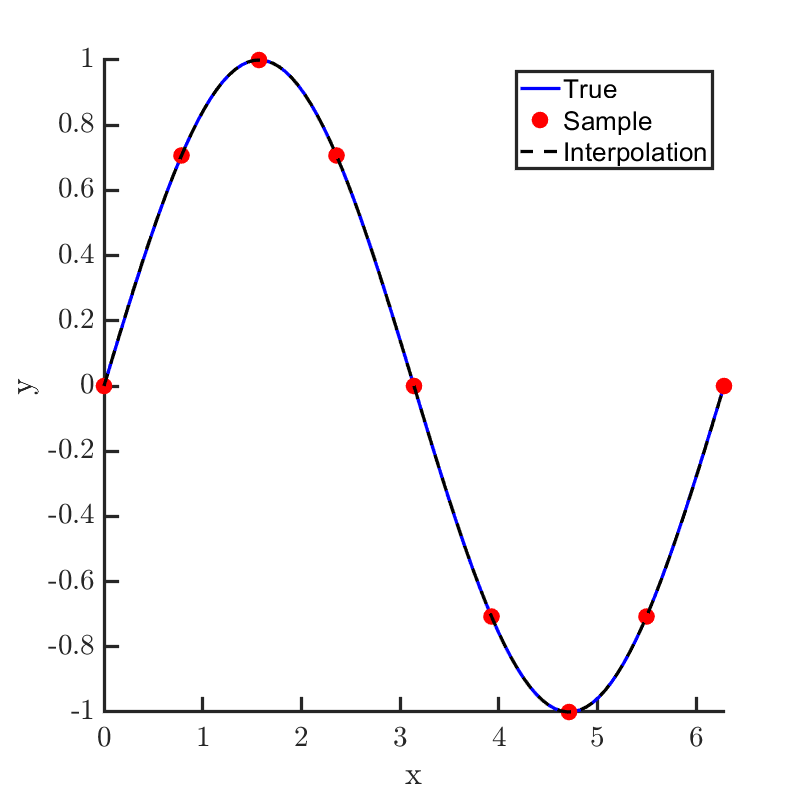
\includegraphics[width=\textwidth]{figs/interp_n8.png}
}    
\end{frame}

\begin{frame}{Runge's Function}
\question{Why was interpolation so bad for $y=\frac{1}{1+x^2}$?}
\cols{
\begin{itemize}
    \item The issue is \textbf{not the function values} --- it is the \textbf{derivatives}

    \item Higher derivatives become \textbf{very large} near the endpoints

    \item So the constant $M$ in the error bound
    \[
    |f^{(n+1)}(x)| \leq M
    \]
    is \textbf{large}

    \item Even if $h$ is small, a large $M$ $\Rightarrow$ large error
\end{itemize}
}
{
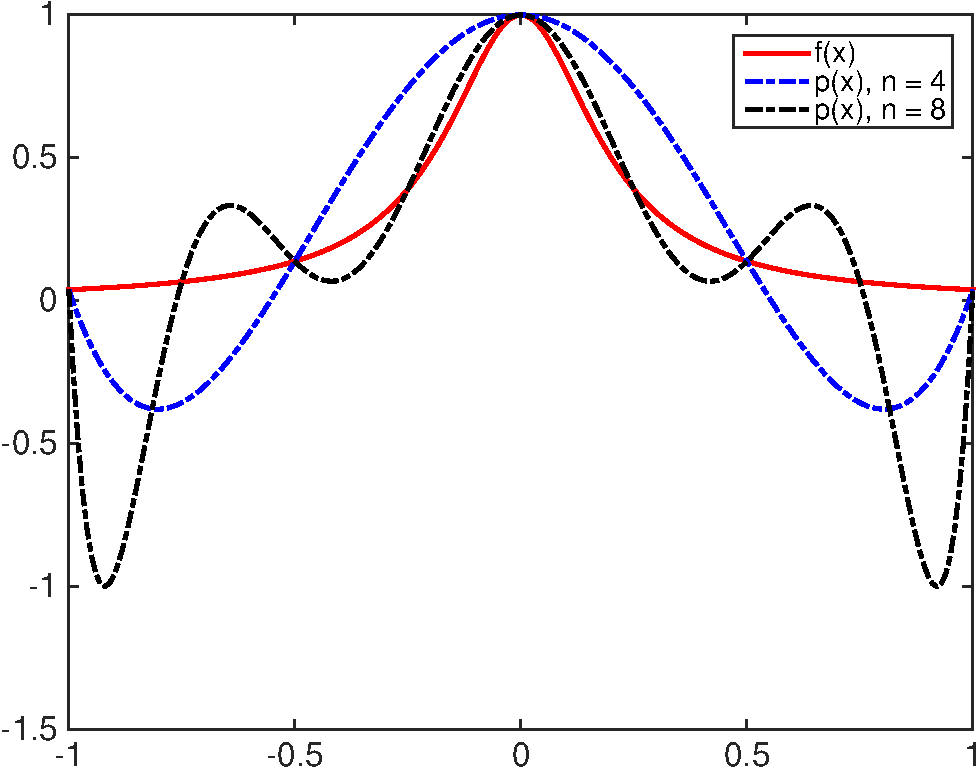
\includegraphics[width=\textwidth]{./figs/runge_interp}
}    
\end{frame}
%%%%%%%%%%%%%%%%%%%%%%%%%%%%%%%%%%%%%%%%
\sectionframe{Chebychev Nodes}
%%%%%%%%%%%%%%%%%%%%%%%%%%%%%%%%%%%%%%%%

\begin{frame}{Issue at the Endpoints}
\vspace{-10mm}
\cols{
\begin{center}
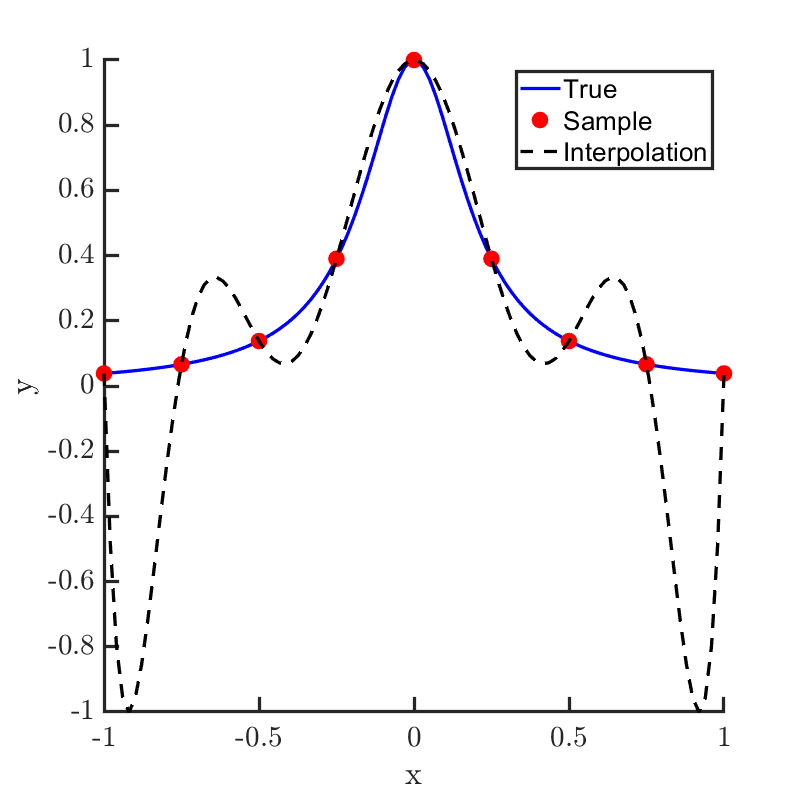
\includegraphics[width=\textwidth]{figs/interp_n8_runge.png}\\
Interpolation with $n=8$
\end{center}

}{
\begin{center}
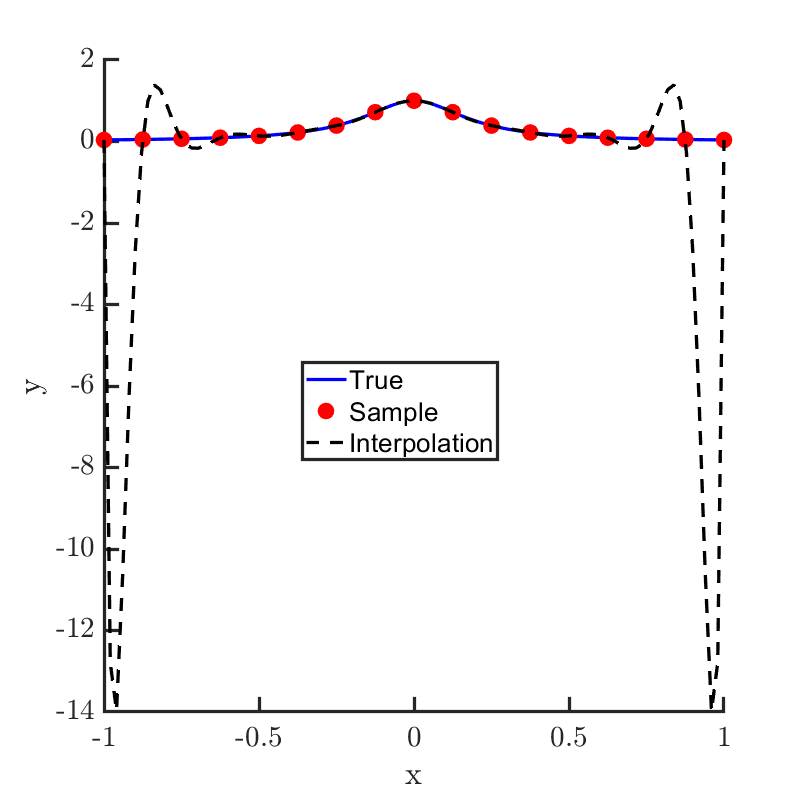
\includegraphics[width=\textwidth]{figs/interp_n16_runge.png}
Interpolation with $n=16$
\end{center}
}
\begin{center}
In Runge's function, the worst error is observed near the endpoints.
\end{center}
\end{frame}




\begin{frame}{Fixes}
We have two options:
\begin{enumerate}
  \item Move the nodes to the problematic areas 
  \item Restrict the maximum order of the polynomial (splines)
\end{enumerate}

\bigskip
\bigskip

Option \#1: Cluster the nodes towards the endpoints
\begin{block}{Chebychev Nodes in $[-1,1]$}    
\begin{equation*}
  x_i = \cos\left(\pi \frac{2i+1}{2n+2}\right), \quad i=0,\dots,n
\end{equation*}
\end{block}
\bigskip
Option \#2: Piecewise polynomials... we discuss later
\end{frame}




\begin{frame}{Chebychev Nodes}
\begin{center}
    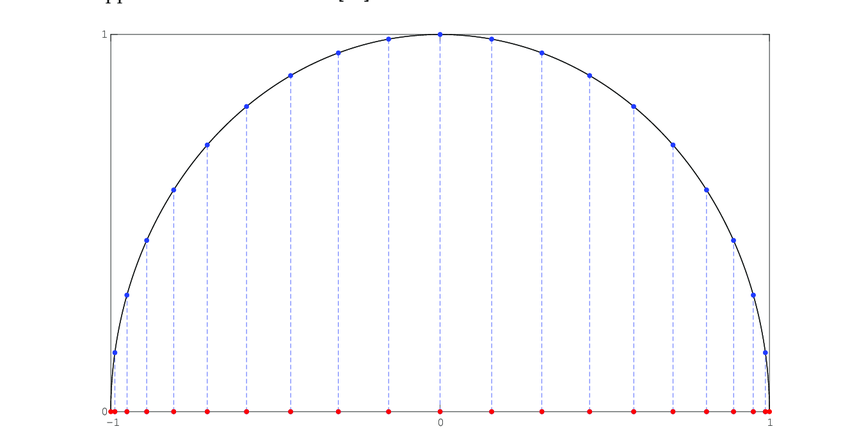
\includegraphics[scale=1.2]{figs/Chebyshev-nodes-proj.png}
\end{center}
\begin{itemize}
\item Nodes from equidistant points on a circle are projected down to the $x$-axis
\end{itemize}
\end{frame}

\begin{frame}
\frametitle{Chebychev Nodes}
\begin{equation*}
  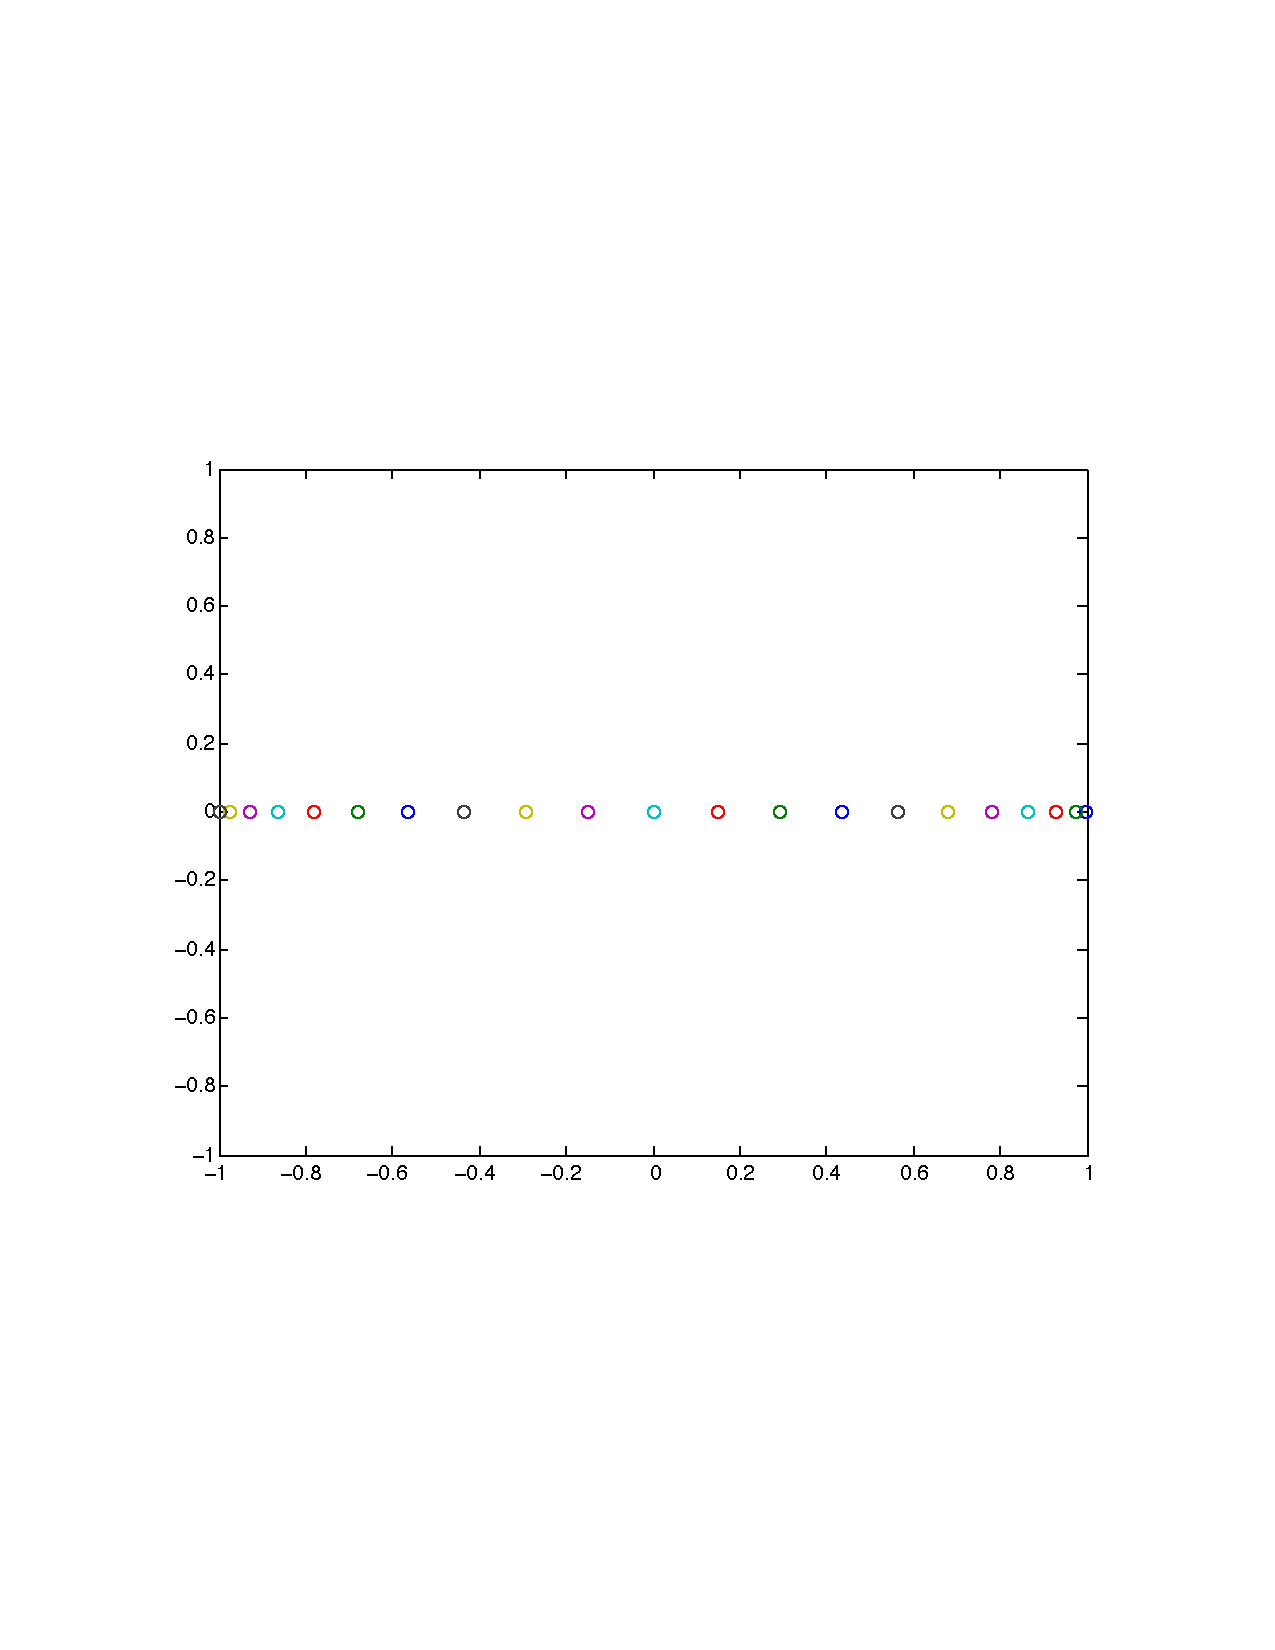
\includegraphics[scale=0.35]{./figs/chebychev}
\end{equation*}
\begin{block}{Key Idea}
\begin{itemize}
    \item With equispaced interpolation, the error is the worst at the endpoints.
    \item Chebyshev lets us systematically create nodes clustered at the endpoints.
\end{itemize}
\end{block}
\end{frame}

\begin{frame}
\frametitle{Chebychev Nodes}
High degree polynomials using equispaced points suffer from many oscillations
\begin{equation*}
  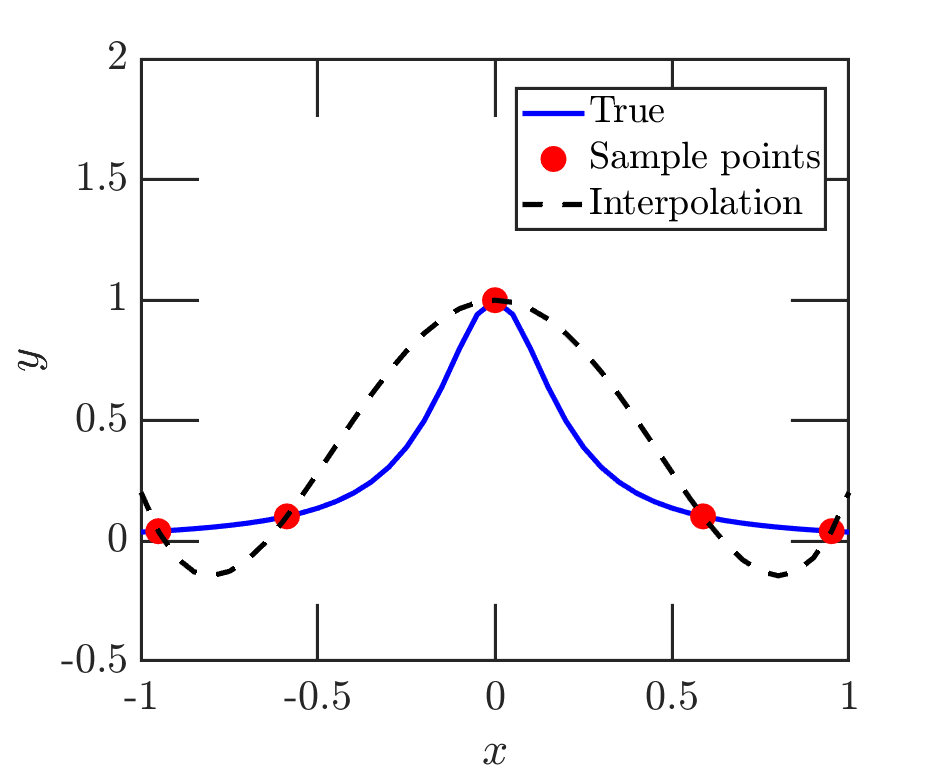
\includegraphics[height=4cm]{./figs/cheb-n4}
\end{equation*} 

\method{Chebychev Sampling}{Interval $[a,b]$, number of points $n+1$}{Set of points $(x_i)$ on $[a,b]$ clustered at endpoints}{Clustering at the ends reduces the error of interpolation}
\end{frame}

\begin{frame}{Is Chebychev the solution?}
\begin{equation*}
  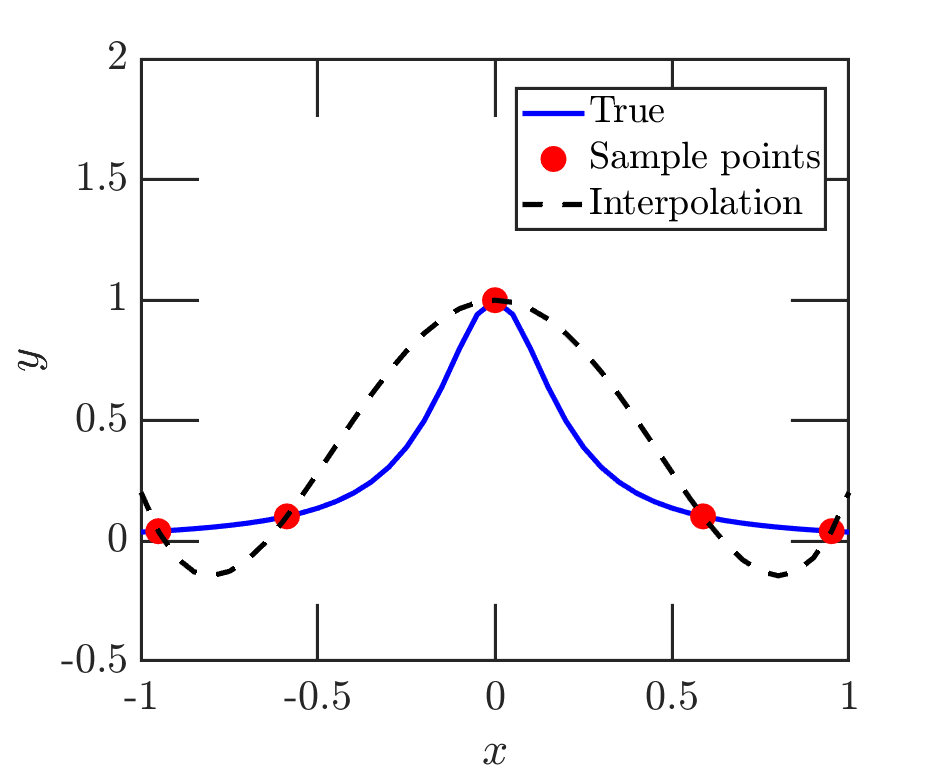
\includegraphics[height=4cm]{./figs/cheb-n4} 
  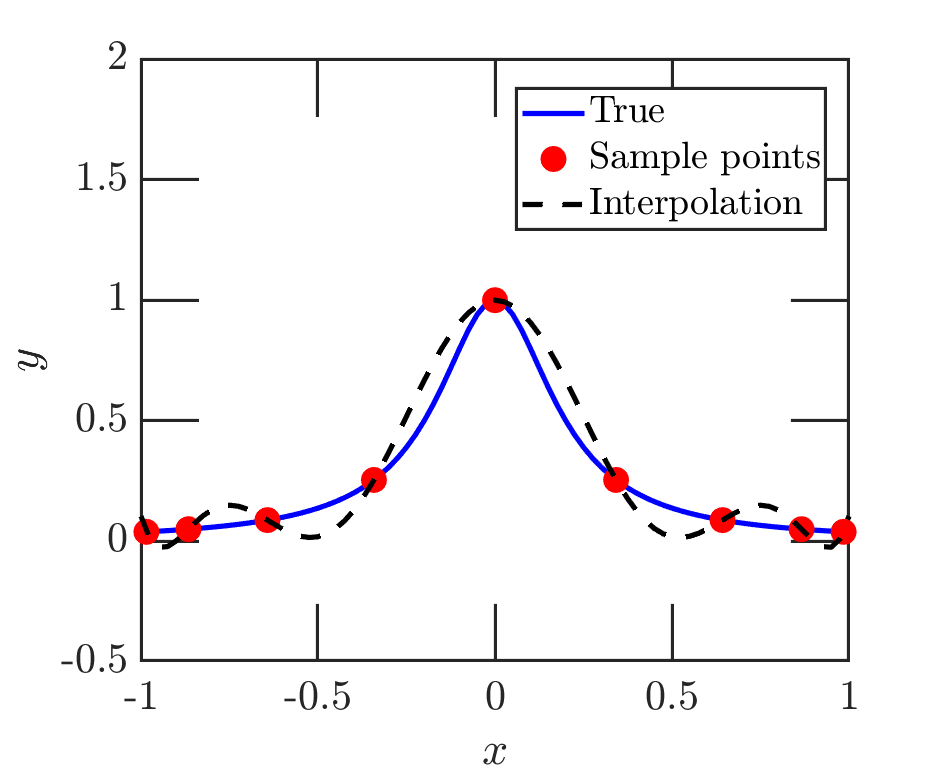
\includegraphics[height=4cm]{./figs/cheb-n8} 
\end{equation*} 
    \begin{itemize}
    \item The figures above shows interpolation with $n=4$ and $n=8$. 
    \question{
        Will Chebychev get better as $n$ increases?\\ 
        Or will it encounter trouble like equispaced interpolation? 
    }
    \onslide<2>{
        \item Homework!
    }
\end{itemize}

\end{frame}

\end{document}

